\subsection{Image Transfer Testing}
\label{subsec:imagetransfertesting}

\begin{figure} [ht]
  \centering
  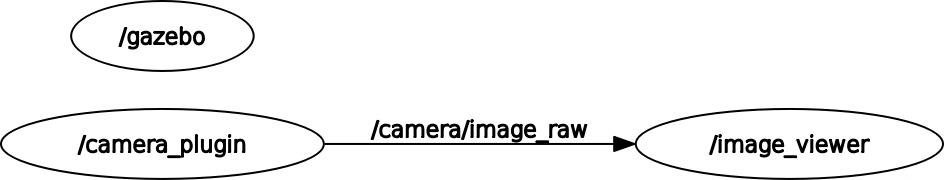
\includegraphics[width=0.45\textwidth]{figures/rosgraph/image-transfer-sim.png}
  \IfLanguageName{english}{
    \caption{Node scheme of the image transfer testing in the simulation.}
  }{
    \caption{Skema \emph{node} dari pengujian pengiriman citra di simulasi.}
  }
  \label{fig:rosgraphimagetransfersim}
\end{figure}

\begin{figure} [ht]
  \centering
  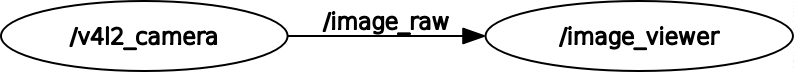
\includegraphics[width=0.45\textwidth]{figures/rosgraph/image-transfer-real.png}
  \IfLanguageName{english}{
    \caption{Node scheme of the image transfer testing in the real robot.}
  }{
    \caption{Skema \emph{node} pengujian pengiriman citra pada \emph{real robot}.}
  }
  \label{fig:rosgraphimagetransferreal}
\end{figure}


Image Transfer Testing is done by running the \lstinline{image_viewer} \emph{node} that will display the received image in the form of GUI.
As shown in figure \ref{fig:rosgraphimagetransfersim},
  in the simulation,
  the \lstinline{image_viewer} \emph{node} will be connected to the \lstinline{camera_plugin} \emph{node} that will send image data using the \lstinline{/camera/image_raw} \emph{topic}.
As for the testing in the real world,
  as shown in figure \ref{fig:rosgraphimagetransferreal},
  the role of the \lstinline{camera_plugin} \emph{node} will be replaced by the \lstinline{v4l2_camera} \emph{node} that will send image data which came from camera device on the real robot.


\begin{figure}[ht]
  \centering
  \begin{tikzpicture}
    \begin{axis}[
        height=0.2\textwidth,
        width=0.45\textwidth,
        xlabel=\IfLanguageName{english}{Data Size}{Ukuran Data} (KB),
        ylabel=\IfLanguageName{english}{Delay}{\emph{Delay}} (ms),
        legend style={
          at={(0.5,1.5)},
          anchor=north,
          legend columns=-1,
        },
        ymajorgrids,
        ymin=0,
        ymax=125,
      ]
      \addplot table[x=size,y=delay,col sep=comma]{data/image-transfer-sim.csv};
      \addplot table[x=size,y=delay,col sep=comma]{data/image-transfer-bd-sim.csv};
      \IfLanguageName{english}{
        \legend{Same Device, Between Device}
      }{
        \legend{Sesama Perangkat, Antar Perangkat}
      }
    \end{axis}
  \end{tikzpicture}
  \IfLanguageName{english}{
    \caption{Delay results of image transfer in the simulation.}
  }{
    \caption{Hasil \emph{delay} dari pengiriman citra di simulasi.}
  }
  \label{fig:imagetransferdelaysim}
\end{figure}


\begin{figure}[ht]
  \centering
  \begin{tikzpicture}
    \begin{axis}[
        height=0.2\textwidth,
        width=0.45\textwidth,
        xlabel=\IfLanguageName{english}{Data Size}{Ukuran Data} (KB),
        ylabel=\IfLanguageName{english}{Rate}{Frekuensi} (hz),
        legend style={
          at={(0.5,1.5)},
          anchor=north,
          legend columns=-1,
        },
        ymajorgrids,
        ymin=0,
        ymax=40,
      ]
      \addplot table[x=size,y=rate,col sep=comma]{data/image-transfer-sim.csv};
      \addplot table[x=size,y=rate,col sep=comma]{data/image-transfer-bd-sim.csv};
      \IfLanguageName{english}{
        \legend{Same Device, Between Device}
      }{
        \legend{Sesama Perangkat, Antar Perangkat}
      }
    \end{axis}
  \end{tikzpicture}
  \IfLanguageName{english}{
    \caption{Rate results compared to the data size of image transfer in the simulation.}
  }{
    \caption{Hasil frekuensi dibandingkan ukuran data dari pengiriman citra di simulasi.}
  }
  \label{fig:imagetransferratesim}
\end{figure}


The image transfer test is carried out under conditions of transmission on the same device and on transmission between two different devices.
Each of these tests is carried out with combinations of resolution values from 160x120 to 1920x1080 on a virtual robot in a simulation environment and on a real robot in the real world.
As shown in figure \ref{fig:imagetransferdelaysim} and figure \ref{fig:imagetransferratesim},
  in the simulation,
  the resulting delay values tends to increase while the resulting rate values tends to decrease with the increase of the sent data.
From these results,
  Up to 800x600 resolution ($\pm2500$ KB),
  image transfer in the simulation could produce low delays under 50 ms and stable rates above 90\% of the normal value.


\begin{figure}[ht]
  \centering
  \begin{tikzpicture}
    \begin{axis}[
        height=0.2\textwidth,
        width=0.45\textwidth,
        xlabel=\IfLanguageName{english}{Data Size}{Ukuran Data} (KB),
        xlabel=\IfLanguageName{english}{$K^{th}$ Attempt}{Percobaan Ke-$K$},
        legend style={
          at={(0.5,1.5)},
          anchor=north,
          legend columns=-1,
        },
        ymajorgrids,
        ymin=0,
        ymax=125,
      ]
      \addplot table[x=size,y=delay,col sep=comma]{data/image-transfer-real.csv};
      \addplot table[x=size,y=delay,col sep=comma]{data/image-transfer-bd-real.csv};
      \IfLanguageName{english}{
        \legend{Same Device, Between Device}
      }{
        \legend{Sesama Perangkat, Antar Perangkat}
      }
    \end{axis}
  \end{tikzpicture}
  \IfLanguageName{english}{
    \caption{Delay results of image transfer on the real robot.}
  }{
    \caption{Hasil \emph{delay} dari pengiriman citra pada robot fisik.}
  }
  \label{fig:imagetransferdelayreal}
\end{figure}


\begin{figure}[ht]
  \centering
  \begin{tikzpicture}
    \begin{axis}[
        height=0.2\textwidth,
        width=0.45\textwidth,
        xlabel=\IfLanguageName{english}{Data Size}{Ukuran Data} (KB),
        ylabel=\IfLanguageName{english}{Rate}{Frekuensi} (hz),
        legend style={
          at={(0.5,1.5)},
          anchor=north,
          legend columns=-1,
        },
        ymajorgrids,
        ymin=0,
        ymax=40,
      ]
      \addplot table[x=size,y=rate,col sep=comma]{data/image-transfer-real.csv};
      \addplot table[x=size,y=rate,col sep=comma]{data/image-transfer-bd-real.csv};
      \IfLanguageName{english}{
        \legend{Same Device, Between Device}
      }{
        \legend{Sesama Perangkat, Antar Perangkat}
      }
    \end{axis}
  \end{tikzpicture}
  \IfLanguageName{english}{
    \caption{Rate results compared to the data size of image transfer on the real robot.}
  }{
    \caption{Hasil frekuensi dibandingkan ukuran data dari pengiriman citra pada robot fisik.}
  }
  \label{fig:imagetransferratereal}
\end{figure}


Meanwhile,
  on the real robot,
  as shown in the figure \ref{fig:imagetransferdelayreal} and figure \ref{fig:imagetransferratereal},
  the obtained results are also relatively the same in which the delay values tends to increase while the rate values tends to decrease.
However,
  different from the test results in the simulation environment,
  from the results on the real robot,
  it is obtained that up to 640x480 resolution ($\pm1500$ KB),
  image transfer on the real robot could produce low delays under 50 ms and stable rates above 90\% of the normal value.
